% Owner: Thuan. ~1.25 pages. Numbers: exps/scf/results/summary.md, results/scf_ablation.md,
% exps/qscf/results/summary.md, paper_acl/sections/analysis.tex (error analysis, 61-run frontier).
\section{Introduction}\label{sec:intro}
In class-incremental learning (CIL) a model learns new classes task after task and must classify every class
seen so far. In the \emph{exemplar-free} setting it may not keep images of past tasks, so whatever it remembers
about an old class has to fit in a compact summary. Methods built on pre-trained vision transformers have made
this setting practical~\cite{l2p,ease,ssiat}. A common recipe trains a light adapter on each task and stores one
mean and one covariance per class~\cite{zhang2023slca,ssiat,rsiat}. RSIAT~\cite{rsiat}, a strong recent
baseline, uses these statistics to correct feature drift and to retrain the classifier on Gaussian samples. Once
the classifier is aligned, however, the statistics play no further role: predictions come from the linear head
alone. Other methods do classify with the statistics, through nearest class means~\cite{zhou2024aper},
Mahalanobis distances~\cite{goswami2023fecam} or a ridge head~\cite{mcdonnell2023ranpac}, but they replace the
trained classifier instead of complementing it.

The same statistics are also a natural input for a quantum model. A class mean and covariance define a density
matrix, and classifying a feature among such states is a problem of quantum state discrimination, for which the
pretty-good measurement (PGM)~\cite{hausladen1994pgm} is a standard choice. Quantum components, however, are
usually judged by inserting them into a strong classical pipeline and reporting a gain of a few tenths of a
point, close to the pipeline's own run-to-run variation, and without a classical model that receives the same
inputs~\cite{bowles2024better,li2026qkd}. Whether the quantum part matters then remains open.

We address both points with \emph{Statistics-Calibrated Fusion} (SCF), shown in Fig.~\ref{fig:pipeline}. SCF
keeps the trained classifier and, at prediction time, adds a second score computed from the stored statistics:
a closed-form ridge classifier or the PGM over class density matrices. The second score is rescaled by a factor
computed from unlabelled training features of the current task, so one fusion weight, chosen once on ImageNet-R
and then frozen, transfers across scores and datasets. SCF needs no extra training of the network and no stored
images. We evaluate it under a protocol designed to resolve small effects: three seeds per benchmark, paired
comparisons with 95\% confidence intervals, every head evaluated on the same trained network, and decision rules
fixed before each experiment. Our contributions are:
\begin{itemize}
  \item \textbf{C1, SCF.} A training-free fusion of the classifier with a statistics-based score. It raises the
        final accuracy of RSIAT by $+0.38$ to $+0.67$ points on CIFAR-100, ImageNet-R, ImageNet-A and CUB-200,
        with the interval above zero on three of them (Table~\ref{tab:main}). The ablation shows that the
        calibration factor turns the mean gain of the ridge score from $+0.14$ into $+0.48$ points
        (Sect.~\ref{sec:ablation}).
  \item \textbf{C2, a quantum measurement with its classical twin.} Every quantum component, at training or at
        prediction time, is compared with a classical model on the same inputs (Table~\ref{tab:twin}). Inside SCF
        the PGM equals ridge ($-0.04$, $[-0.17,+0.08]$, 12 paired runs). Three propositions explain why: circuits
        after the encoding, shrinkage of the states and rescaling of the score cannot change the prediction
        (Sect.~\ref{sec:props}).
  \item \textbf{C3, why fusion helps.} The linear head and the PGM make different errors: they disagree on
        14\% of ImageNet-R test images, and each is right on a different part of them. Fusion therefore raises accuracy on old and new classes
        together, whereas every training-time change we tried trades one for the other (Sect.~\ref{sec:why}).
        A pre-registered $2\times2$ experiment confirms this: SCF adds $+0.38$ and $+0.44$ points of average
        accuracy on classically and quantum-trained networks, while quantum training adds $+0.09$,
        $[-0.08,+0.26]$, once SCF is used (Sect.~\ref{sec:qscf}).
\end{itemize}

\begin{figure}[t]
\centering
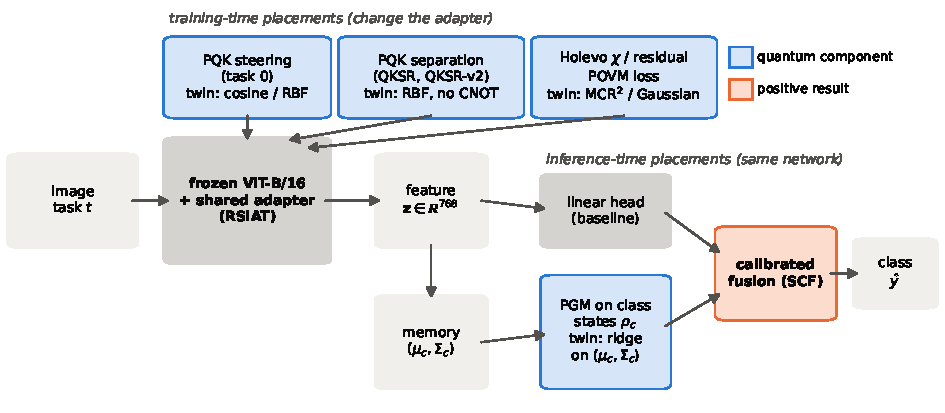
\includegraphics[width=\textwidth]{figures/pipeline.pdf}
\caption{\TODOD{Placeholder figure from the ACL version. Redraw it in the order of the Method section,
left to right: (1) training: image $\to$ ViT+adapter, PQK on the base task and QKSR on incremental tasks
(small, faded box); (2) memory $(\mu_c,\Sigma_c)$; (3) inference (main, highlighted box):
$z$ $\to$ linear head $\|$ (memory $\to\rho_c\to$ PGM, or ridge) $\to$ fusion with $\kappa$ $\to\hat y$.
You can edit \texttt{paper\_acl/make\_figures.py}, function \texttt{pipeline()}.}}
\label{fig:pipeline}
\end{figure}
